\documentclass[12pt, a4paper]{article}
\usepackage{graphicx}
\usepackage{fourier}
\usepackage{indentfirst}

\title{\Huge Cloud Databases}
\author{\Large Leon Radó}
\date{\today}

\begin{document}

\maketitle
\begin{figure}[b]
    \centering
    
\includegraphics[width=0.8\linewidth]{images/STU-FIIT.png}
\end{figure}
\thispagestyle{empty}

\clearpage
\tableofcontents

\clearpage
\begin{abstract}
    The following article provides a brief overview of cloud computing, especially databases. Firstly, it describes the main principles of cloud databases, their history, differences with standard on-premises databases, and options of implementation. Later, the reader will learn about different types of databases, their benefits, challenges, and concerns. In this section essential properties of cloud databases like cost-effectiveness, flexibility, accessibility, and maintenance are compared. Afterwards, this writing introduces leading cloud database providers and the services they offer, for example, Amazon Web Services (AWS), Google Cloud, Microsoft Azure, and others. In the end, it mentions the latest trends in cloud computing like serverless databases as well as the future of cloud databases. After reading this paper, the reader will gain basic knowledge of database systems and understand the importance and rising popularity of cloud computing.\\\\
    \footnotesize{
        \textbf{Keywords:}
        \textit{database, cloud computing, relational database, nosql, cloud provider}
    }
\end{abstract}
\clearpage

\section{Introduction}
    A cloud database is a particular type of database that works just like a standard on-premise database system but differs by its type of placement. While traditional databases exist on physical servers, cloud databases operate in a cloud environment. That means the database system is not located in the business infrastructure, but instead, it is accessible via the cloud by a specific cloud service provider. \textit{Cloud computing has become the norm of the today's computing world. This paradigm shift is looking for the databases that are compatible in all respect.}\cite{03} Each of these two types has an advantage over the other in terms of cost-effectiveness, accessibility, performance, security, and many other important characteristics, so it is up to the business owner to choose the right option for the purpose and requirements of his business. \par In this article, I will mainly focus on the benefits and concerns that come with cloud databases to understand how these new types of databases work and what improvements they can offer to the world of data management.
\clearpage

\section{Cloud Database Implementation}
    There are two primary methods to implement a cloud database, the thing they have in common is the presence of a third-party cloud service provider. One of these options is operating the database on the cloud independently of the provider with the virtual machine. Another option is using the database as a service (DBaaS).
    
    \subsection{Virtual Machine Image}
        Providers allow users to create a virtual machine image to directly access a database stored on the cloud. This virtual machine includes the database software, operating system, and necessary configurations.\par The owner pays for the specific resources he needs, the cost is predictable and based on the resources and services he selects. This type of implementation requires manual and more demanding management but offers better control of the database and more options for customization.
    
    \subsection{Database as a Service}
        DBaaS is a more commonly used method to implement a cloud database. This service provides a database for the user through the Internet and includes hosting, setup, and management of the system, so the user doesn't have to worry about additional complex work related to maintaining a database. \textit{Enterprises may focus on their core competencies instead of having to maintain complex IT landscapes.}\cite{11}\par DBaaS most often follows a pay-as-you-go pricing method, which means the owner pays just for the resources utilized at the moment.
        \begin{figure}[b]
            \centering
            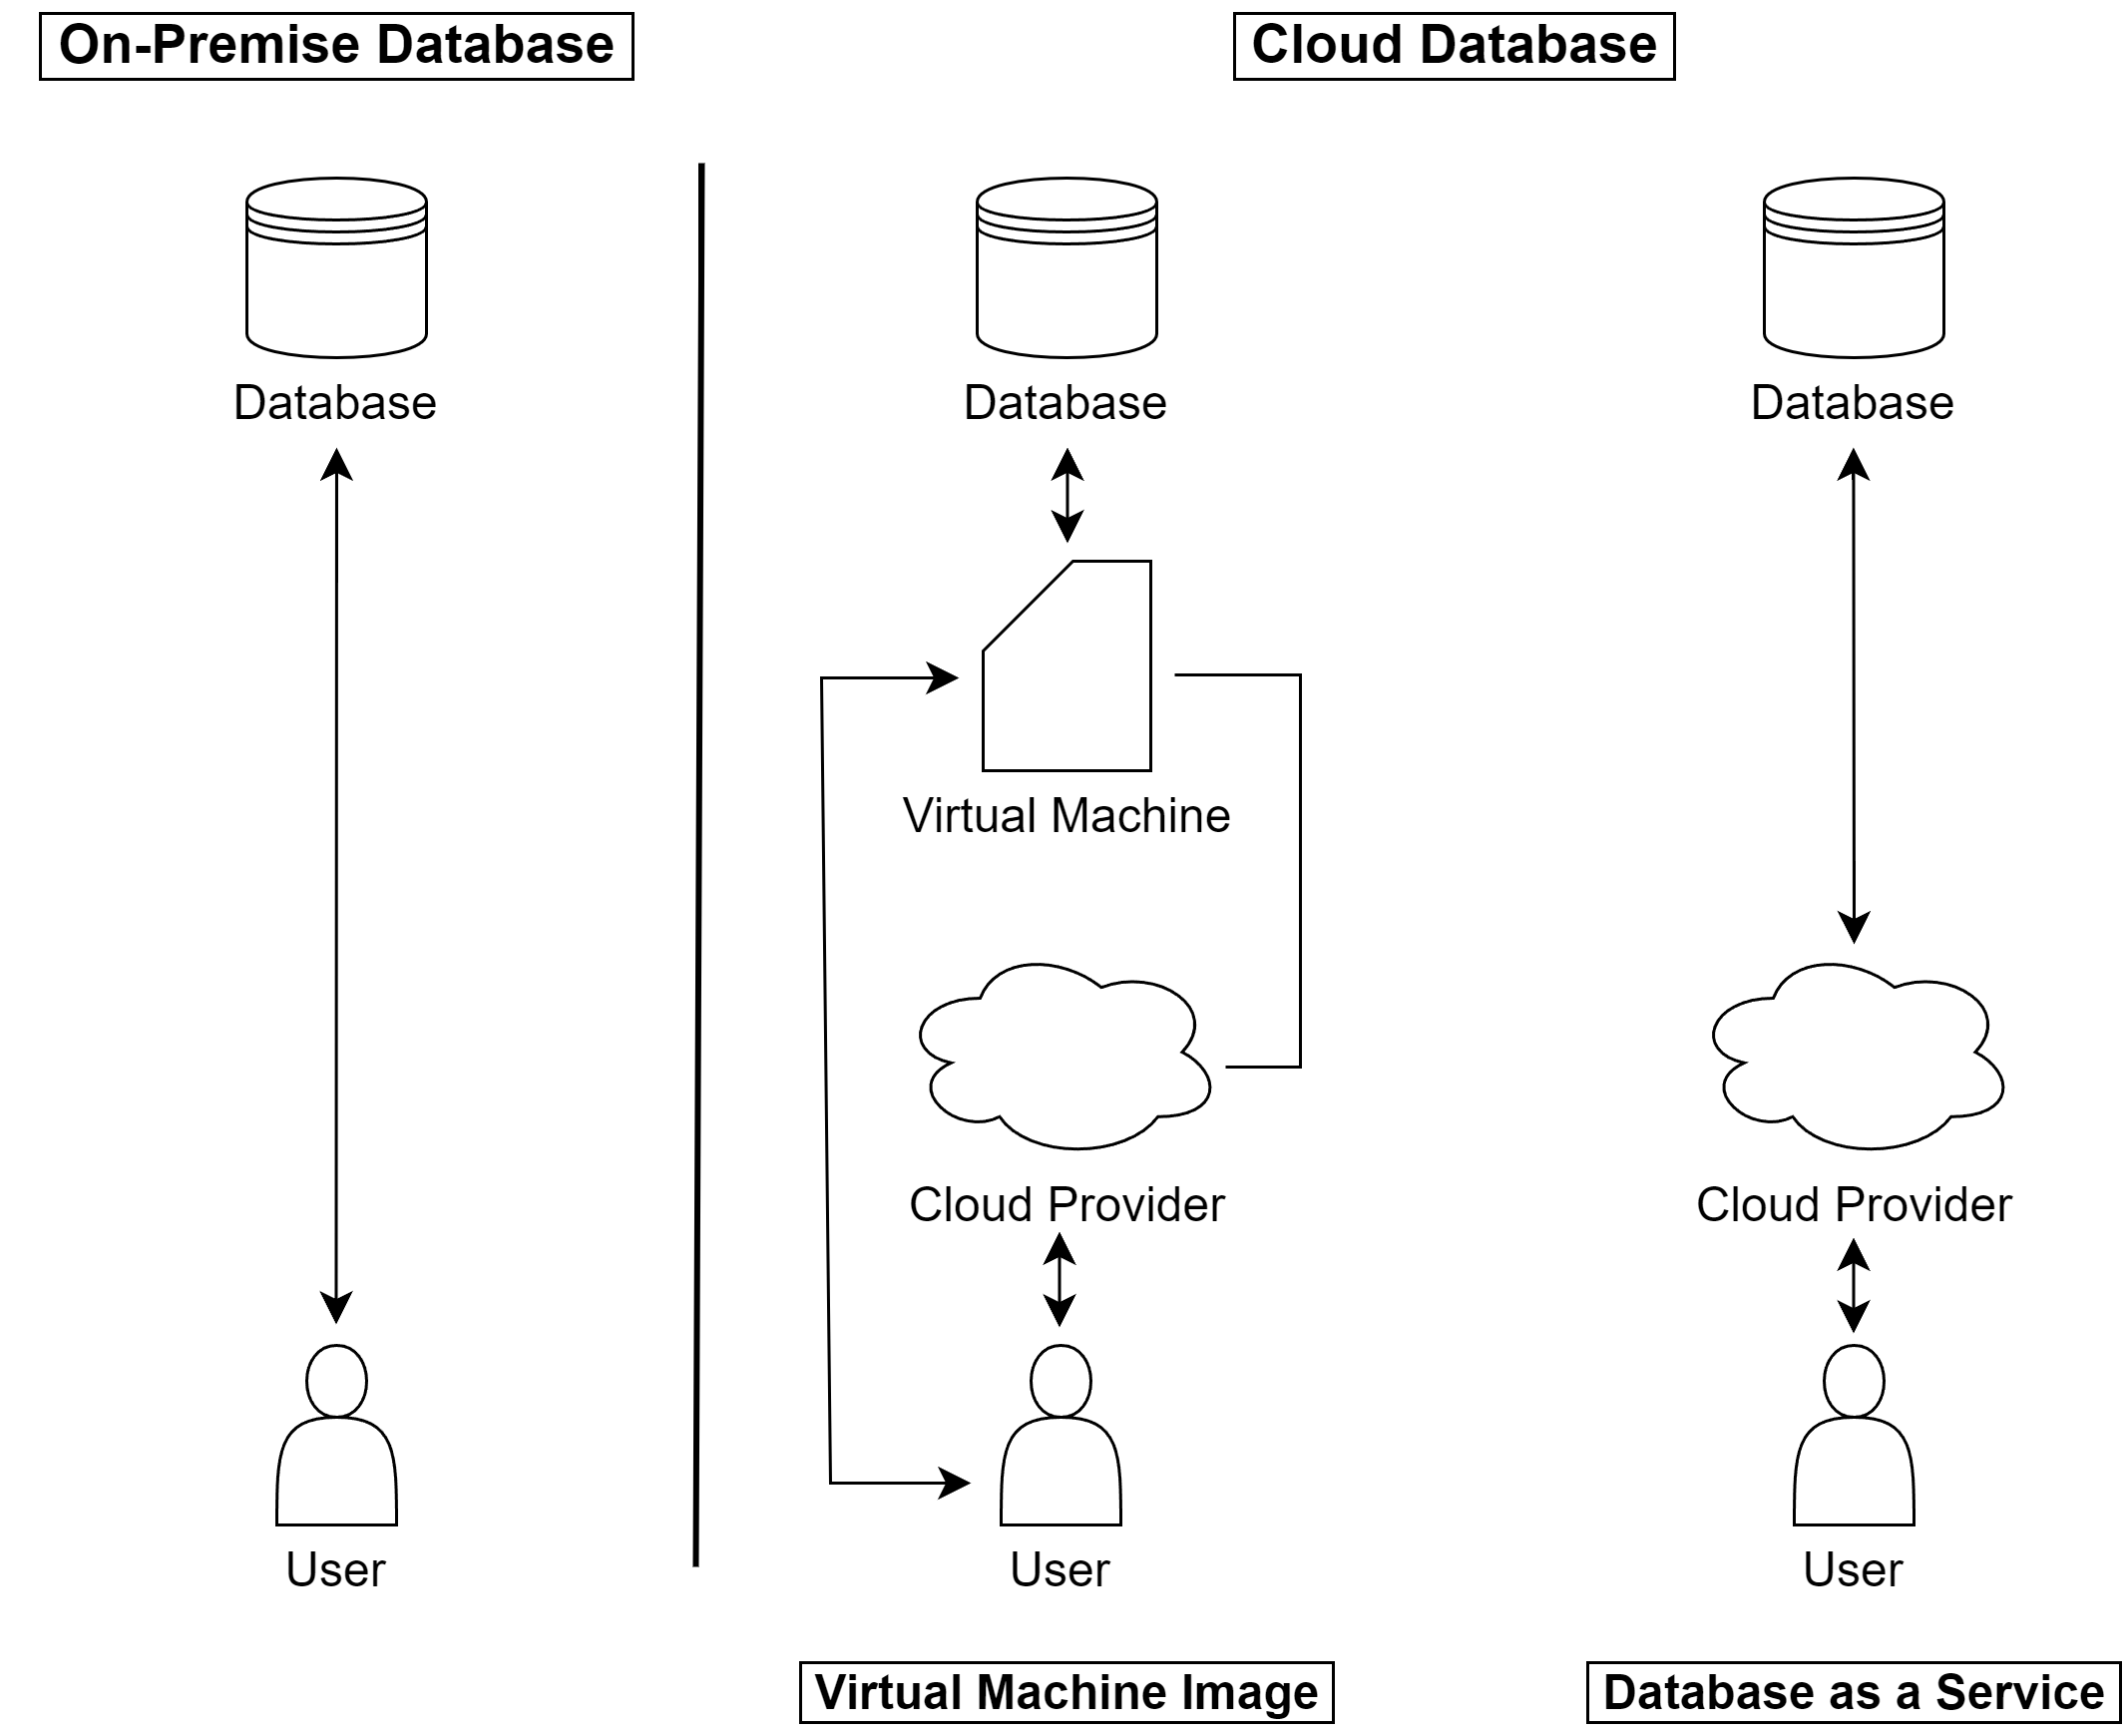
\includegraphics[width=1\linewidth]{images/onpremise-cloud.png}
            \caption{Comparison of Database Systems}
            \label{fig:comparison}
        \end{figure}
\clearpage

\section{Types of Cloud Databases}
    Just like standard on-premise databases, cloud databases can be divided into relational databases and non-relational, usually referred to as NoSQL databases. When choosing the right database it's important to consider the strengths, weaknesses, and use cases of both types.

    \subsection{Relational Databases}
        These databases store structured information organized into rows and columns, the structure of the data has to be defined in advance. Relation databases are typically used for applications with structured data, for example, transactional systems, and offer consistency and reliability, however, they are usually scaled vertically, which means they can be demanding on server resources like CPU and RAM.

    \subsection{NoSQL Databases}
        Non-relational databases are designed to work with a large amount of unstructured data, that is most often stored in key-value pairs without predefined format. This type of database is adequate for example for web applications that store a variety of information. \textit{NoSQL databases were born to meet performance needs, leaving other details like atomicity in the background.}\cite{06}\\
        \begin{figure}[h]
            \centering
            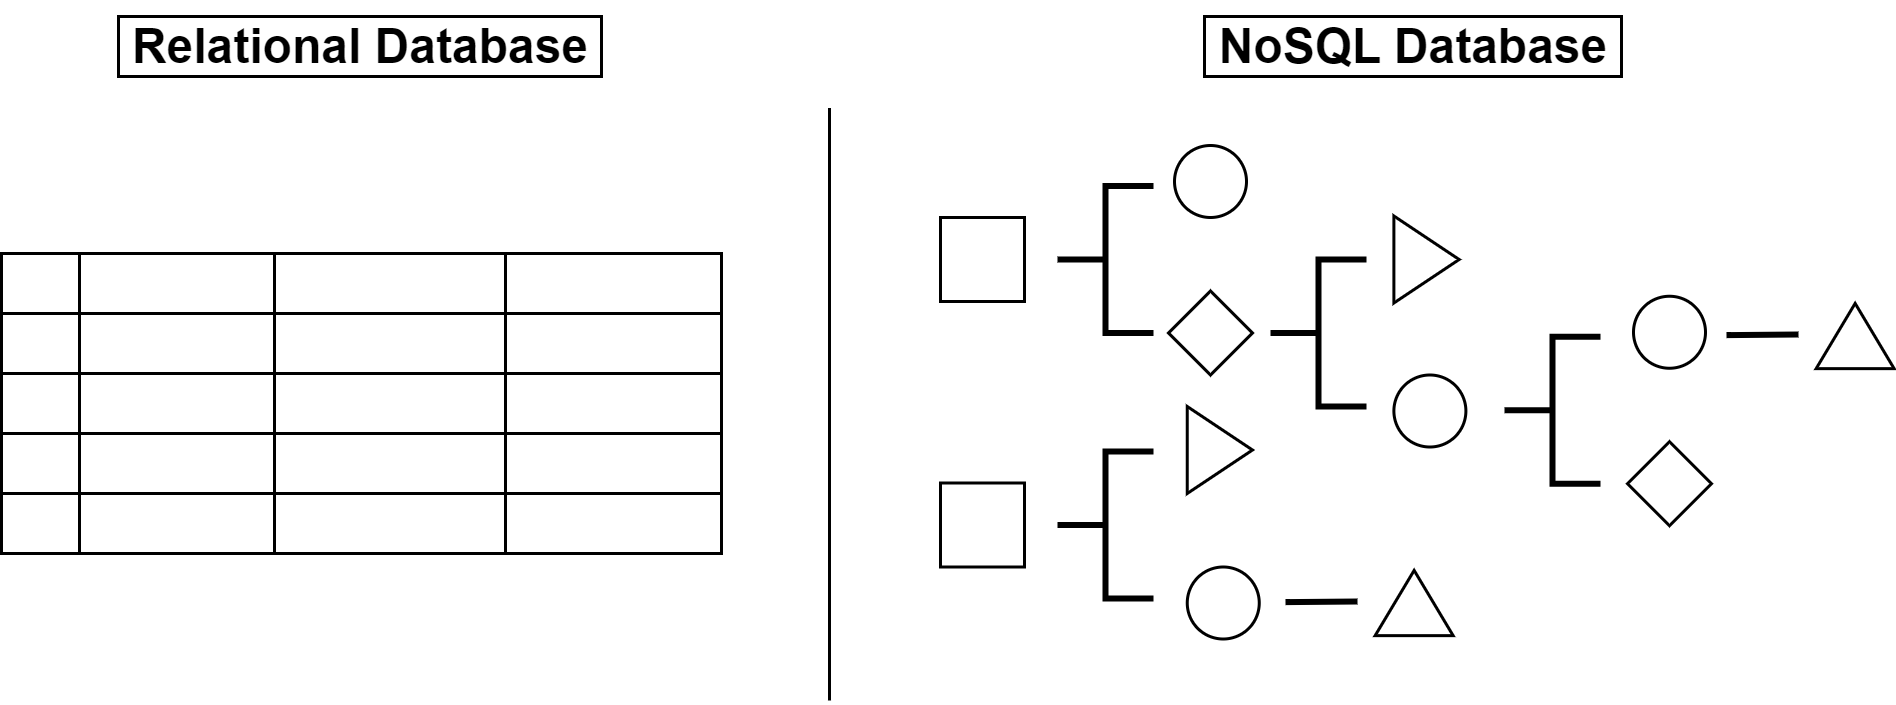
\includegraphics[width=1\linewidth]{images/relational-nosql.png}
            \caption{Structure of Relational and NoSQL Database}
            \label{fig:structure}
        \end{figure}
\clearpage

\section{Benefits of Cloud Databases}
    \subsection{Accessibility}
        Accessing a cloud database isn't limited by geographical location and can be done from anywhere with a stable Internet connection. This feature is especially useful for organizations that need access to the database from different locations.
    
    \subsection{Scalability}
    \subsection{Managed Services}
    \subsection{Cost-Efficiency}
    \subsection{Disaster Recovery}
\clearpage

\section{Concerns of Cloud Databases}
    \subsection{Data Security}
    \subsection{Network Dependency}
    \subsection{Vendor Lock-In}
    \subsection{Limited Control}
\clearpage

\section*{}
\clearpage
\bibliographystyle{unsrt}
\bibliography{refs}

\end{document}
